%\documentclass{article}
\documentclass[twocolumn]{article}
\usepackage[utf8]{inputenc}
\usepackage{graphicx}

\title{IFT6390 Project1}
\author{Marthy Garcia, Rafael Garcia}
\date{March 2021}

\begin{document}

\maketitle

\section{Introduction}
This paper report on the design and documentation of a machine learning model, as a part of a Introduction to Machine learning course at the University of Montreal. 

Our main task is to predict the mean per capita (100,000) cancer mortalities for a given set of details about US counties. In this document, the authors describe the pre-processing of data, model selection, testing, hyper-parameter tuning, and validation.

\section{Data } \label{secData}

The data used in this project can be found in \cite{bibdata}. The data has various attributes about the US counties, cancer rates, resident characteristics distribution.The train data-set comprises 32 features and 3047 observations containing numerical and categorical variables. The full data dictionary can be found in \cite{bibdatadict}.

Features with more than 50\% missing values were dropped (e.g."pctsomecol18\_24"). On numerical variables missing values were replaced by the mean of the fields. Categorical variables did not have missing values.

\subsection{Training and test data sets} \label{secsplit}
The original data was split in training and testing data set. As advised in \cite{bibDangeti2017},  20\% of the data was randomly selected for testing, the remaining data was assigned to training.

\section{Pre-processing steps} \label{secpre}
An exploratory data analysis (EDA) that comprised correlation and distribution analysis was performed on the training data set to inform model selection. Figure \ref{fig:corr} depicts the correlation matrix. Multiple variables show a strong correlation within them. As an example, the mean per capita cancer mortalities has a positive relationship with the median income per county. As per Figure \ref{fig:corr}, the median income per county is highly correlated multiple variables as well. This indicates that we should perform feature selection before implementing a model.

\begin{figure}
    \centering
    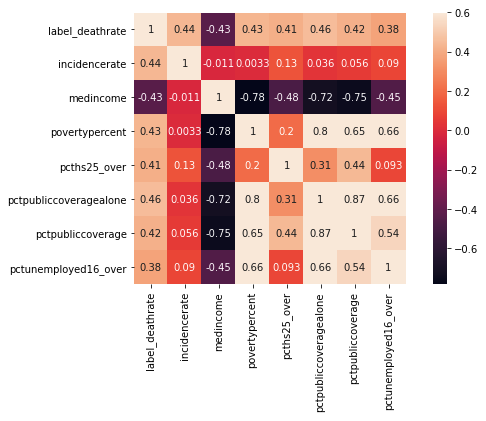
\includegraphics[width=7cm]{correlation.png}
    \caption{Correlation matrix}
    \label{fig:corr}
\end{figure}

Figure \ref{fig:linear} shows the target variable against the feature: \% of country residents with public coverage.  The latter depict a linear relationship. The same behaviour is observed with multiple features. A linear regression seems promising.

\begin{figure}
    \centering
    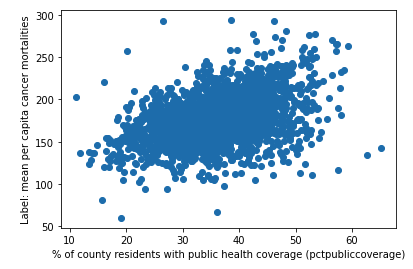
\includegraphics[width=7cm]{linearrelation.png}
    \caption{Target variable vs \% of country residents with public coverage}
    \label{fig:linear}
\end{figure}

Must of the numerical variables follow skewed distributions and have different scales. Therefore, logarithmic transformation was applied to improve our model fit and score. Logarithmic transformation increased the accuracy of the model by almost 60\%. Categorical variables were transformed using one-hot encoding. 

\section{Model Selection}\label{secmodel}

\subsection{Hyper-parameter tuning} \label{secpar}
As per Figure \ref{fig:rfe}, some features exhibit a high correlation. Feature selection was done by applying a grid search Recursive Feature Elimination (RFE) cross-validation. A 10- fold cross-validation was selected. Models were compared based on the $R^2$. Figure \ref{fig:rfe} shows the $R^2$ value as a function of the number of features. A total of 15 feature were selected.

\begin{figure}
    \centering
    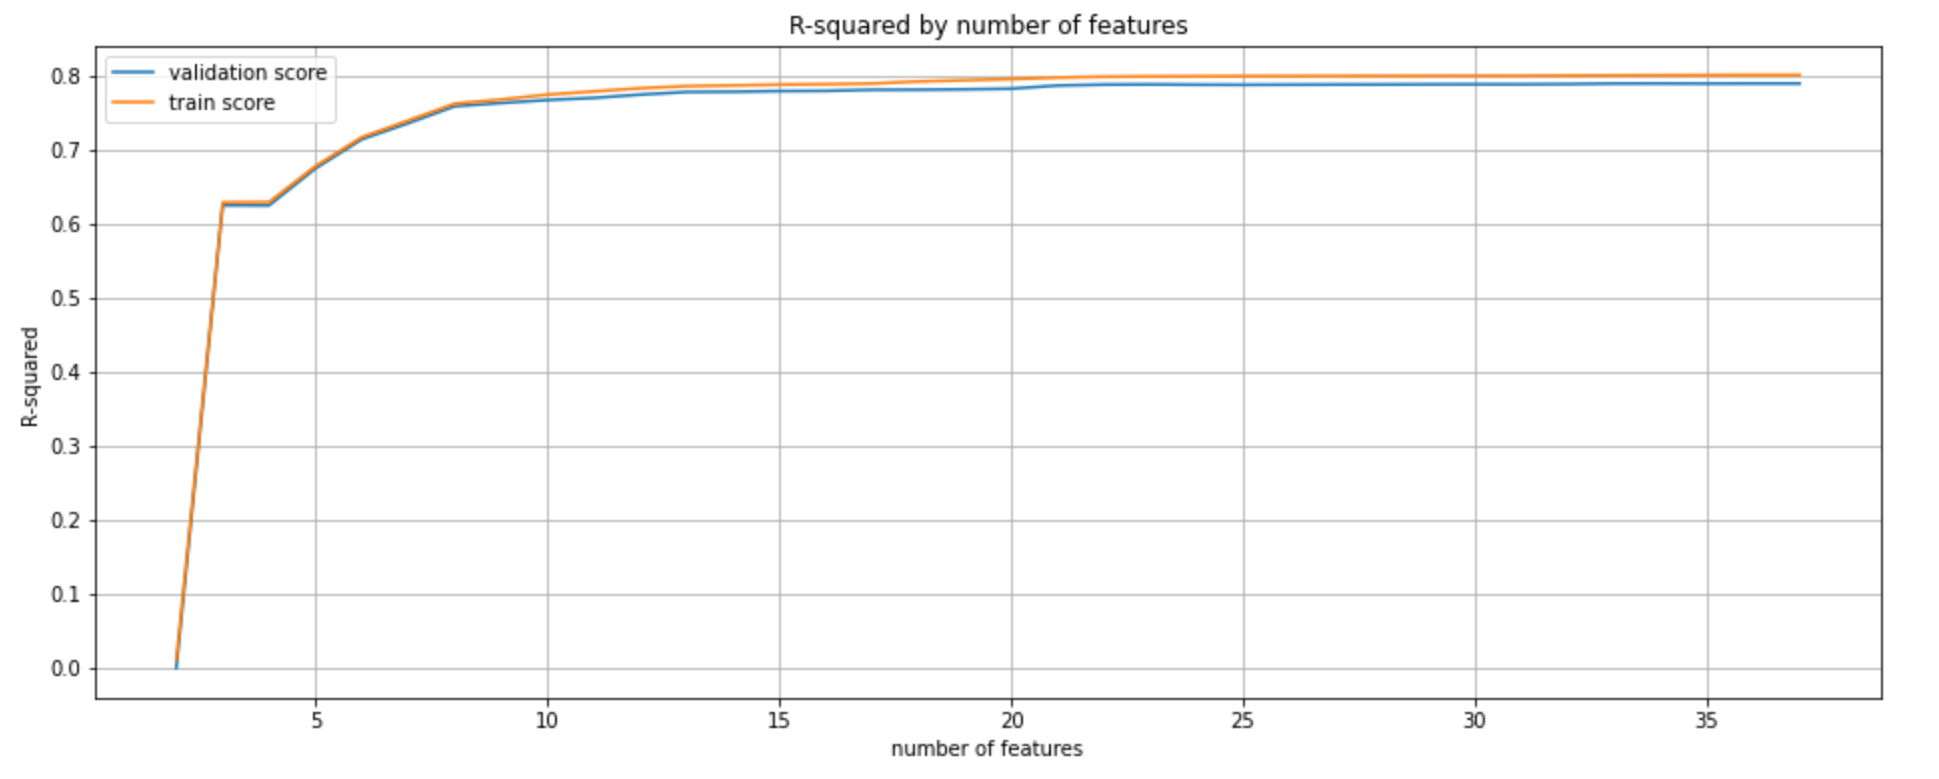
\includegraphics[width=7cm]{RFE.png}
    \caption{$R^2$ by number of features}
    \label{fig:rfe}
\end{figure}

\subsection{Linear Regression}
 Linear regression is a method that finds the best linear fit to a given independent and dependent variables. The best fit is found by minimizing the sum of squared residuals.
 
 As per the findings from Figure \ref{fig:linear}, a linear regression method was chosen as per its simplicity, interpretability, and simple implementation. The model is given as follow:
 
 $$Y=XA+E$$
 Where
 
 \[X=\left[ \begin{array}{cccc}
1 & x_{1,1}  &...&x_{1,15}\\
1 & x_{2,1}  &...&x_{3,15}\\
\vdots & \vdots &...&\vdots\\
1 & x_{n,1} &...&x_{n,15}
\end{array} \right]
%
Y=\left[ \begin{array}{c}
y_{1} \\
y_{2} \\
\vdots \\
y_{n}
\end{array} \right]
%
E=\left[ \begin{array}{c}
e_{1} \\
e_{2} \\
\vdots \\
e_{n}
\end{array} \right]
\]
The matrix $A$ consist of the weight of each feature. We solve for $A$ as follows:
$$A=(X^TX)^{-1}X^TY$$ \label{eqA}
\subsection{Time and space complexity}
As per \cite{{bibBanerjee20}} the training complexity of the model is $O(k^2(n+k))$. Where $k$ corresponds to the number of features.
The test runtime complexity of linear regression is $O(k)$

The training space complexity is $O(nk+n)$. The test space complexity at run time is $O(k)$.

The model was run in Colab free version. Figure \ref{fig:fittime} shows the run time per fold. The average fit time is 0.106s with a standard deviation of 0.019.  

\begin{figure}
    \centering
    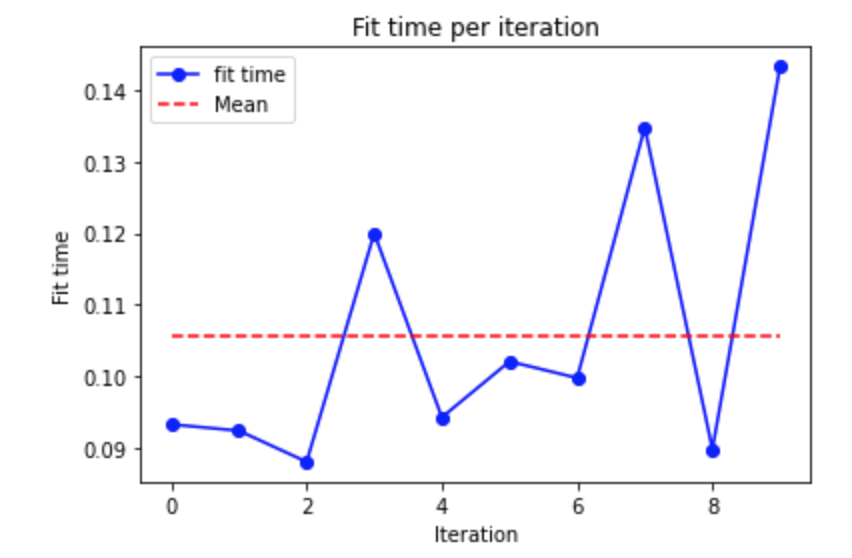
\includegraphics[width=7cm]{fittime.png}
    \caption{Fit time per fold}
    \label{fig:fittime}
\end{figure}

\section{Model score}\label{secscore}
To ensure reproductivity of the results, a seed was set in all steps.

Performance was validated by applying a 10- fold cross-validation and measured by the $R^2$. Figure~\ref{fig:rsqrd_trainval} shows the $R^2$ value for the training and validation sets. The test $R^2$ obtained is 0.775. The Mean Absolute Error (MAE) and the Mean Squared Error (MSE) were also collected. Table~\ref{tabresults} summarize the results for the training, validation and test data sets.

\begin{center}\label{tabresults}
\begin{tabular}{ |c|c|c|c|c| } 
 \hline
 Set   &mean $R^2$ &std.dev $R^2$   & MAE   & MSE \\
 \hline
 Train      &0.787      & 0.041                     &0.053  &0.005 \\ 
 Valid &0.778      &0.041                      &0.054  & 0.054\\ 
 Test       & 0.775     &-                          &0.054  & 0.072\\ 
 \hline
\end{tabular}
\end{center}

\begin{figure}
    \centering
    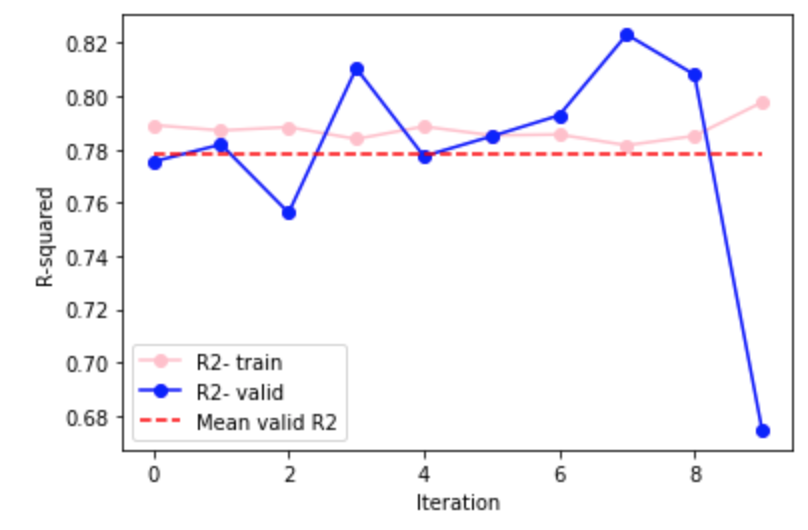
\includegraphics[width=7cm]{r_sqdtrainvalid.png}
    \caption{Train and validation $R^2$ per fold}
    \label{fig:rsqrd_trainval}
\end{figure}

\section{Conclusion and further work}\label{secconclusion}

The objective of this model is the prediction of the mean per capita (100,000) cancer mortalities. We performed the following steps as an iterative process: feature engineering (pre-processing), feature selection and model selection. 

Logarithmic transformation of numerical variables significantly increase the performance of our model. An initial EDA, showed a high correlation between the variables. Hence, RFE was applied to select the most important features. A linear regression was built. Cross-validation helped to create a more robust model by no creating a validation set.

This project had limitation in the gathering of additional information. We recommend further work focused on collecting additional features.


%%%%%%%%%%% References%%%%%%%%%%%%%%%%%%%%%%%%%%
\begin{thebibliography}{100} % 100 is a random guess of the total number of %references

\bibitem{bibdata}
Linear Regression Exercise 1: Data word

\bibitem{bibdatadict} 
Linear Regression Exercise 1- metadata: Data word,\texttt{https://data.world/exercises/linear}

\bibitem{bibDangeti2017} Dangeti, Pratap, ``Statistics for Machine Learning: Techniques for Exploring Supervised, Unsupervised, and Reinforcement Learning Models with Python and R," 2017, \emph{Packt Publishing}

\bibitem{bibBanerjee20}
Banerjee, Writuparna,``Train/Test Complexity and Space Complexity of Linear Regression," 2020,\texttt{https://levelup.gitconnected.com/}

\end{thebibliography}
%%%%%%%%%%%%% end %%%%%%%%%%%%%%%%%%%%%%%%%%%%%%%


\end{document}
